\chapter{Analyse des Besoins et Modélisation}

\section{Identification des Acteurs}
Le système interagit principalement avec trois profils d'utilisateurs distincts. L'Étudiant est l'utilisateur central, consommant les cours, dialoguant avec l'agent IA et se soumettant aux évaluations. L'Enseignant endosse le rôle de créateur de contenu, de validateur des examens générés et d'arbitre final face aux alertes de fraude. L'Administrateur supervise la plateforme, gère les habilitations et s'assure du bon fonctionnement technique de l'infrastructure.

\section{Diagrammes de Cas d'Utilisation}

La modélisation UML permet de formaliser les interactions entre les acteurs et la plateforme. Le diagramme global ci-dessous illustre l'architecture fonctionnelle de haut niveau de la solution Fraudly.

\begin{figure}[h!]
    \centering
    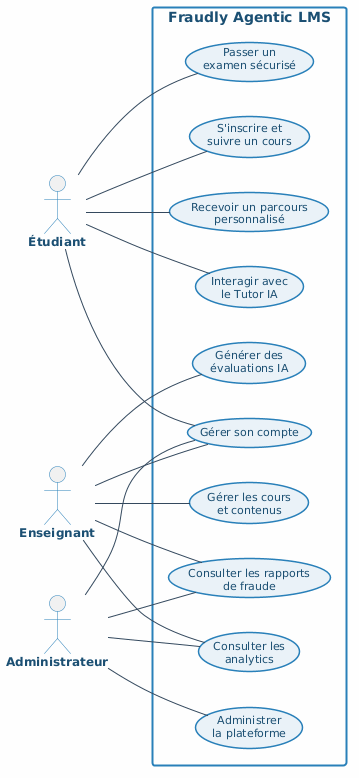
\includegraphics[max width=\textwidth, max height=0.4\textheight, keepaspectratio]{../UC01_Globale.png}
    \caption{Diagramme de Cas d'Utilisation Global}
    \label{fig:uc_global}
\end{figure}

L'étudiant s'authentifie sur la plateforme, consulte ses parcours d'apprentissage personnalisés, et participe aux sessions d'évaluation sous la surveillance automatisée du module de proctoring. 

\subsection{Service d'Authentification}
Le processus d'authentification centralise le contrôle d'accès. La figure \ref{fig:uc_auth} détaille les opérations d'inscription, de connexion sécurisée et de gestion de profil.

\begin{figure}[h!]
    \centering
    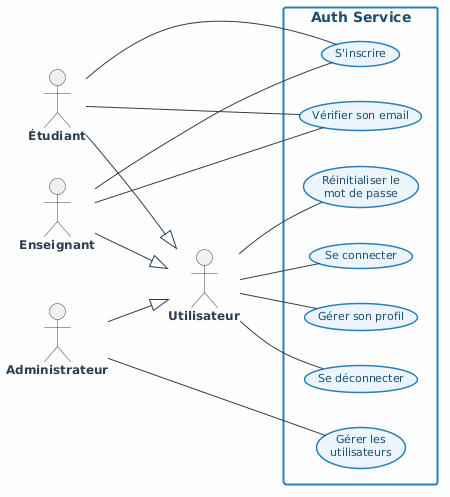
\includegraphics[max width=\textwidth, max height=0.4\textheight, keepaspectratio]{../UC02_Auth_Service.png}
    \caption{Cas d'Utilisation du Service d'Authentification}
    \label{fig:uc_auth}
\end{figure}

\subsection{Service de Cours (Learning Hub)}
Le cœur de la gestion pédagogique est confié au service de cours. L'enseignant y téléverse ses ressources, tandis que l'étudiant y navigue guidé par l'IA.

\begin{figure}[h!]
    \centering
    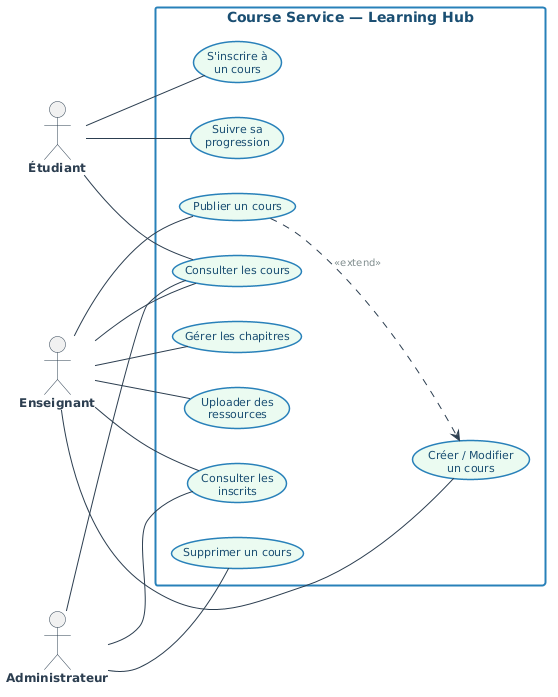
\includegraphics[max width=\textwidth, max height=0.4\textheight, keepaspectratio]{../UC03_Course_Service.png}
    \caption{Cas d'Utilisation du Service de Cours}
    \label{fig:uc_course}
\end{figure}

\subsection{L'Agent d'Intelligence Artificielle}
Le service d'intelligence artificielle expose les fonctionnalités agentiques : tutorat, génération d'examens et correction. La figure \ref{fig:uc_ai} schématise ces interactions avancées.

\begin{figure}[h!]
    \centering
    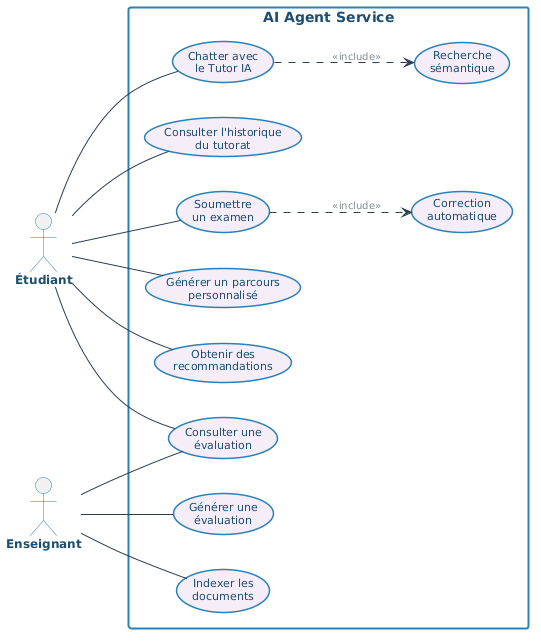
\includegraphics[max width=\textwidth, max height=0.4\textheight, keepaspectratio]{../UC04_AI_Agent_Service.png}
    \caption{Cas d'Utilisation de l'Agent IA}
    \label{fig:uc_ai}
\end{figure}

\subsection{Le Service de Proctoring}
Le module de télésurveillance, crucial pour le projet, est représenté par la figure \ref{fig:uc_proctoring}. Il illustre la capture des flux vidéo, l'analyse comportementale et la génération de rapports d'intégrité.

\begin{figure}[h!]
    \centering
    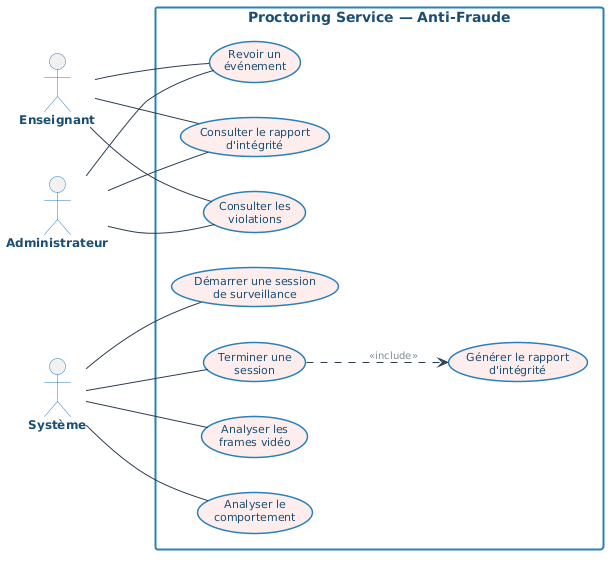
\includegraphics[max width=\textwidth, max height=0.4\textheight, keepaspectratio]{../UC05_Proctoring_Service.png}
    \caption{Cas d'Utilisation du Service de Proctoring}
    \label{fig:uc_proctoring}
\end{figure}

\section{Spécifications Non Fonctionnelles}
Au-delà des fonctionnalités, la plateforme Fraudly doit répondre à des critères d'exigence critiques. La sécurité des données personnelles et académiques exige l'utilisation de protocoles de chiffrement forts et d'une authentification par jetons JWT. La scalabilité est impérative pour supporter la charge des milliers d'étudiants se connectant simultanément lors d'épreuves d'examen. Enfin, la performance du moteur de proctoring vidéo requiert une latence minimale pour assurer l'équité et l'efficacité de la surveillance.
